\label{sex:kink}
\index{Sex!kink|(}
\fontspec{Gentium Book Basic}[Color=EEEEEEFF,Ligatures=TeX]
\renewfontfamily\allyFont{Merriweather Sans}[Scale=0.9,Color=EEEEEEFF,Ligatures=TeX]

\noindent What do you do when you've got a libido and relatively little will to act upon it?

Delve into kink.

\begin{ally}
Well, and fuck around on Taps a lot.\index{Sex!TS}
\end{ally}
The two go hand in hand. When sex makes you intensely anxious, it turns out that getting tied up and blindfolded just sort of multiplies that anxiety.

\begin{ally}
So you removed yourself from the equation.
\end{ally}
Close enough, yes. I let my characters bear the weight of kink and sexual interaction. Textually, there's a vast divide between what's on the screen and what's going on in person. I can get all I need from kink without actually needing to interact with it.

\begin{ally}
And what do you need from kink?
\end{ally}
Beyond just fantasy fulfillment? A way to cope, I suppose.

\noindent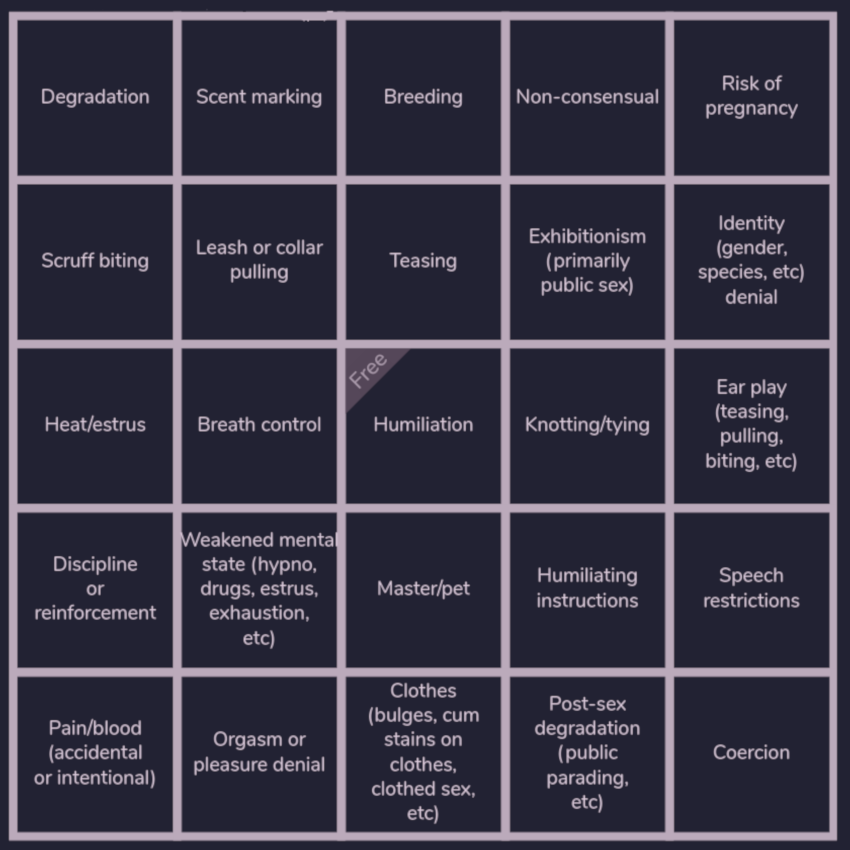
\includegraphics[width=2.5in]{assets/static/sex/kink/bingo.png}

\begin{ally}
I'm not really sure what to make of the fact that you made a bingo card for your kinks.
\end{ally}
Well, hey, hit bingo, and maybe I explode or something. Besides, \emph{bbbingo} was for a game jam.

\begin{ally}
So tell me about your free space.
\end{ally}
Actually, I think many of them come from a similar space: recasting bad or uncomfortable experiences from childhood into some positive light. A way to reclaim them and make them positive again.

\begin{ally}
How is humiliation positive?
\end{ally}
Okay, maybe some of them are not so much `again'.

\begin{ally}
I don't imagine non-consensual sex ever was, no.
\end{ally}
Not really, but using kink as a coping mechanism for anxieties around rape is at least a way forward for me.

Ditto humiliation. Being made to feel inadequate, often by people I was supposed to look up to, was such a negative force in my life --- in Matthew's life\index{The Death of Matthew} --- that it left me with quite a bit of baggage. This is just a way to sort through it.

\begin{ally}
Sexily.
\end{ally}
I suppose. It's something of a metakink. Many of the others stem from that, or from a similar core interest.

Scent-play as a means of degradation: why would a snow leopard smell of canine? Fits in nicely with knotting. Why not toss in some species denial, too; no more kitty, you say `arf' now. Good dog, good pet, you belong to master.\index{Relationships!Justin}\index{Furry}

Scruffing, in the context of furry, especially with felines, is a means of rendering one helpless. Coercion and weakened mental states fit as well. Those all sort of tag along with the non-consensual core kink.

\begin{ally}
So, pain and blood? Breathplay?
\end{ally}
Yes. Abuse. Damage. Bad ends.

\begin{ally}
Where do those come from?
\end{ally}
Self hatred. Self harm. Destroy me before I destroy myself.\index{Mental health!self harm}

\begin{ally}
Really?
\end{ally}
No, of course not.

\begin{ally}
But some part of you actively believes that? Some part of you actively craves someone destroying you? Beating you bloody? Choking you? Leaving you for dead with casual nonchalance?
\end{ally}
Yes.
\newpage

\begin{ally}
Do you enjoy vanilla sex, then?
\end{ally}
Perhaps. I suppose I must. So much of what I did for so long, online and off, was vanilla. Even now, much of it is.\index{Sex!TS}\index{Furry}

\begin{ally}
Yet ``sneps are for abusing''.\index{Furry!fursoñas!Maddy}
\end{ally}
Yes.

\begin{ally}
Why?
\end{ally}
I enjoy vanilla sex. It feels good. All this kink, though, helps me grow. It's exposure therapy.

It was exposure therapy when a TS partner on Taps laughed in my face as he raped me and left me to clean myself up. It is exposure therapy because I can say no, because I can enjoy being tied up now.

It was exposure therapy when I was ordered to describe what I wanted in lurid detail. It's exposure therapy because I can talk about sex now.

It was exposure therapy when I entered into a few master/pet relationships. It's exposure therapy because at some point I was able to handle a power-dynamic in my relationships.

It was exposure therapy when I spent scene after scene toying with fertility. It's exposure therapy because at some point I was able to deal with the idea of not being cis, of motherhood being unattainable.

It was exposure therapy when I made my character a pudgy nerd and still able to engage with her sexually. It's exposure therapy because I've been able to come to terms with my body.

\begin{ally}
It's exposure therapy because at some point, you started enjoying sex --- or at least enjoying it more --- and the thought of sharing that with someone.
\end{ally}
Yes.
\newpage
\index{Sex!kink|)}
